\section{Additional Related Work}
\label{sec.more_rw}

\subsection{Benchmarking Coding Agents} 
The past two years have seen the emergence of comprehensive benchmarks to evaluate autonomous code-writing and code-fixing agents on realistic tasks. One prominent example is SWE-Bench \citep{swebench}, which poses real-world GitHub issues and provides the full repository context; an agent succeeds by producing a patch that passes all project tests. 
It has since evolved into a family of benchmarks targeting different scenarios: for instance, variants like SWE-Bench-Multilingual \citep{yang2025swesmith} and SWE-Bench-Multimodal \citep{yang2025swebench} extend the evaluation to codebases with multiple programming languages and to tasks that involve not only code but other modalities (such as modifying documentation or configurations), respectively. An expanded challenge, SWE-Bench Pro \citep{sbp}, was released to assess long-horizon problem solving: it includes complex, enterprise-level issues that may require dozens of files to be modified across a codebase. These benchmarks have become a driving force for the community, with public leaderboards spurring rapid progress. Beyond bug-fixing, entirely new benchmarks are probing other dimensions of software work. SWE-fficiency \citep{ma2025swe} is a recent benchmark that challenges agents to optimize the runtime performance of real codebases given defined workloads. 
% In summary, a rich benchmarking ecosystem now exists for software engineering AI, and it highlights a gap between what current LLM agents can do and the full spectrum of a professional developer’s skill set.

\subsection{Large-scale Software Engineering}
Modern software engineering at scale has driven interest in AI assistance that can handle massive codebases and performance-critical systems. Potvin and Levenberg’s seminal description of Google’s single vast code repository illustrates the challenges and benefits of the monorepo model \citep{potvin2016google}. This approach centralizes billions of lines of code, enabling unified tooling and refactoring, but it demands automated support for code discovery, understanding, and consistent changes at scale. Recent LLM-based systems are beginning to tackle such issues. For instance, Lin et al. introduce ECO, an LLM-driven code optimizer designed for warehouse-scale computers \citep{lin2025eco}. ECO leverages a code-generating model to suggest performance improvements in large distributed software, aiming to reduce runtime and resource usage while preserving correctness. Early results show that AI-powered optimization can uncover non-trivial efficiency gains in complex systems, hinting at a future where coding agents assist not only in writing code but also in optimizing and maintaining it across ultra-large codebases. The combination of monorepo development and LLM-based tools like ECO underscores a trend toward holistic scale: treating an entire organization’s code as a single evolvable system, with AI agents providing the intelligence to manage global changes, dependency analysis, and performance tuning in ways humans alone could not easily scale. This context also motivates advanced context management techniques – instead of feeding billions of lines directly into an LLM, agents must learn to retrieve and focus on the relevant project fragments, a theme that connects to memory and tool-use innovations discussed later.

\subsection{Training LLMs for Software Engineering} 
SWE-Gym \citep{pan2024training} provides the first publicly available executable environment tailored for real-world software engineering tasks: it bundles complete Python repositories with dependencies, unit tests, and realistic issue descriptions, enabling agents to propose patches which can be validated via execution. Later, SWE-Smith \citep{yang2025swesmith} generalizes the idea: given any Python repository, it automatically generates hundreds to thousands of new bug-fix or issue-resolution tasks by perturbing code or simulating realistic faults, producing a dataset of around 50,000 instances across 128 GitHub projects. Training on this large-scale synthetic data significantly improves agent performance on benchmark tasks, indicating that domain-specific, execution-aware fine-tuning is critical for bringing coding agents closer to real-world software engineering demands.
Recent research have explored reinforcement learning for code agents. SWE-RL \citep{wei2025swe} takes advantage of the abundant software evolution data in open-source repositories – commit histories, diff patches, and issue resolutions – and uses these as implicit demonstrations to fine-tune an LLM via RL. The insight is that by learning from how human developers iteratively improve code over many commits, an agent can internalize more realistic problem-solving trajectories. Early results from SWE-RL show improved reasoning and success rates on long-horizon software tasks, as the RL-trained model learns to recover intermediate reasoning steps (e.g. the decision to run tests or check certain files) that are often needed for complex bug fixes.




\section{Context Summarization Ablations}
\label{app:context}
The architect agent summarizes its working memory during execution when it exceeds given threshold; we evaluate whether the quality of context summarization affects downstream agent performance.
In this ablation, we fix the summary \emph{format}, and approximately keep the summary \emph{length}, and \emph{summarization cadence} in comparable ranges, and vary only the LLM used to generate summaries.
All runs use the same main orchestrator (Claude~4~Sonnet) and are evaluated on SWE-Bench Pro.
We compare Claude~3.5~haiku and Claude~4~Sonnet as summarizers.
haiku is chosen as the ``weak'' model because it reliably produces well-formed, schema-compliant summaries, while being substantially weaker in reasoning ability: on SWE-Bench, haiku achieves 40.6\% versus Sonnet’s 72.7\%, and lacks extended multi-step reasoning, hence this choice avoids confounding effects from malformed summaries or instruction non-compliance.

We select 50 long-context instances in which summarization is triggered at least once during execution (up to five times in the longest cases).
Under identical conditions, haiku-based summarization resolves 22/50 instances, while Sonnet-based summarization resolves 26/50. The observed gap directly demonstrates that higher-fidelity, reasoning-capable summaries provide better guidance for subsequent planning and lead to higher final resolve rates.

To illustrate why the quality of the summarization matters, here we provide summary examples of \texttt{instance\_gravitational\_\_teleport-db89206db6c2969266e664c7c0fb51b70e958b64}.

Here is the context summary of Claude Haiku 3.5: 
\begin{tcolorbox}[colback=white,  % background color
                   colframe=black,    % frame color
                   coltext=metablue,      % text color
                   breakable,
                   fontupper=\scriptsize\fontfamily{pcr}\selectfont]  % font style and size
\begin{verbatim}
<summary>
 [CONVERSATION CONTEXT]
- Initial Requirements: Replace fatal error handling in TSH CLI commands with 
error return mechanisms
- Scope Changes: Modify command handlers to return errors instead of calling 
utils.FatalError
- User Preferences: Maintain existing logging and error handling patterns while 
improving test environment flexibility

[TECHNICAL DECISIONS]
- Architecture Decisions: Convert command handler functions to return errors
- Technology Stack: Go language, Teleport client library
- Design Patterns: Error wrapping using trace.Wrap(), trace.BadParameter()
- APIs/Interfaces: Modify function signatures in tool/tsh/tsh.go and 
lib/client/api.go

[IMPLEMENTATION PROGRESS]
- Completed Work: 
  * Added SSOLoginFunc type
  * Modified ssoLogin method
  * Updated onSSH, onPlay command handlers
  * Started modifying onLogin and onLogout
- Current State: Partial implementation of error handling refactoring
- failed Attempts: Initial attempts to replace utils.FatalError with simple 
return statements
- Debugging History: systematic approach to replacing error handling across 
multiple files

[TECHNICAL Details]
- Data Structures: CLIConf, Config structs modified
- Algorithms: Error propagation and wrapping
- Edge Cases: Handling various error scenarios in CLI commands
- Performance Considerations: Minimal performance impact, improved testability

[OUTSTANDING ITEMS]
- Known Issues: Incomplete error handling in complex functions like onLogin
- Open Questions: How to handle early returns in long functions
- TODOs: Complete error handling for remaining command handlers
</summary>
<plan>
 <thinking>
  - Problem Analysis: Complex error handling refactoring across multiple files
- Impact Assessment: Improved testability and error management in Teleport CLI
- Solution Strategy: systematic conversion of command handlers to return errors
 </thinking>
 <issues>
  1. utils.FatalError calls prevent programmatic error handling
2. Complex functions with multiple error points need careful refactoring
3. Function signatures must change to support error returns
 </issues>
 <next_step sequence_num="1">
  Complete error handling conversion for onLogin function
- Replace all utils.FatalError calls with return trace.Wrap(err)
- Handle early return cases by returning nil or specific errors
- Ensure function signature returns error
 </next_step>
\end{verbatim}
\end{tcolorbox}
Here is the summary of Claude Sonnet 4:
\begin{tcolorbox}[colback=white,  % background color
                   colframe=black,    % frame color
                   coltext=metablue,      % text color
                   breakable,
                   fontupper=\scriptsize\fontfamily{pcr}\selectfont]  % font style and size
\begin{verbatim}
<summary>
 [CONVERSATION CONTEXT]
- Initial Requirements: Fix TSH login and proxy address handling for test 
environments by making CLI commands return errors instead of exiting, supporting
mock SSO login injection, and using runtime-assigned addresses for services 
bound to `:0`
- Scope Changes: None - requirements remained consistent throughout
- User Preferences: systematic approach with todo.md planning, focus on minimal 
changes, backward compatibility

[TECHNICAL DECISIONS]
- Architecture Decisions: Chose to implement error returns instead of process 
termination for all command handlers, added pluggable SSO login interface
- Technology Stack: Go, existing Teleport codebase structure maintained
- Design Patterns: Used function type for SSO login injection, trace.Wrap for 
error propagation
- APIs/Interfaces: Defined SSOLoginFunc type with specific signature matching 
existing ssoLogin method

[IMPLEMENTATION PROGRESS]
- Completed Work: 
  * Phase 1: Added SSOLoginFunc type, MockSSOLogin field to Config struct, 
mockSSOLogin field to CLIConf struct
  * Partial Phase 2: Updated refuseArgs helper and several command handlers 
(onLogout, onListNodes, onListClusters, onSSH) to return errors
- Current State: In middle of Phase 2, about to update Run function in Phase 3
- failed Attempts: None significant
- Debugging History: None required yet

[TECHNICAL Details]
- Data Structures: Added SSOLoginFunc type, MockSSOLogin field to Config, 
mockSSOLogin field to CLIConf
- Algorithms: Error propagation using trace.Wrap, replacing utils.FatalError and
os.Exit calls
- Edge Cases: Handling exit status preservation in SSH command, ambiguous host 
error handling
- Performance Considerations: Minimal impact, just changing error handling flow

[OUTSTANDING ITEMS]
- Known Issues: None identified yet
- Open Questions: Need to complete remaining command handlers and service 
address binding logic
- TODOs: Complete Phase 2 (remaining command handlers), Phase 3 (Run function), 
Phase 4 (SSO mock), Phase 5 (service binding), Phase 6 (validation)
</summary>
<plan>
 <thinking>
  - Current State: Successfully implemented Phase 1 (new types/interfaces) and 
partially completed Phase 2 (error handling for some command handlers)
- Architecture Implications: The error handling changes are fundamental and 
affect the entire CLI flow
- Risk Assessment: Need to ensure all command handlers are updated consistently 
and the Run function properly handles all error cases
 </thinking>
 <next_step sequence_num="1">
  Update the Run function signature to return error and modify the switch 
statement to capture errors from all command handlers, including updating the 
refuseArgs call for logout and replacing utils.FatalError with proper error 
return
 </next_step>
\end{verbatim}
\end{tcolorbox}

The summary format and token count are almost identical between the 2 summaries, while Sonnet 4 appears much better in quality. The "[CONVERSATION CONTEXT]" of sonnet preserves maximum information: ``Fix TSH login + proxy handling for test environments by returning errors instead of exiting...", while the haiku summary ``Replace fatal error handling with error returns." loses important keywords.
Most notably, Sonnet shows phases of work: \textbf{it specifies state of the system (Phase 1 done, Phase 2 mid-way, next is Run function)}, making progress legible and actionable..

\section{Meta-Agent}
\subsection{Implementation Details}
\label{sec.meta-agent-details}
\begin{figure*}[t]
    \centering
    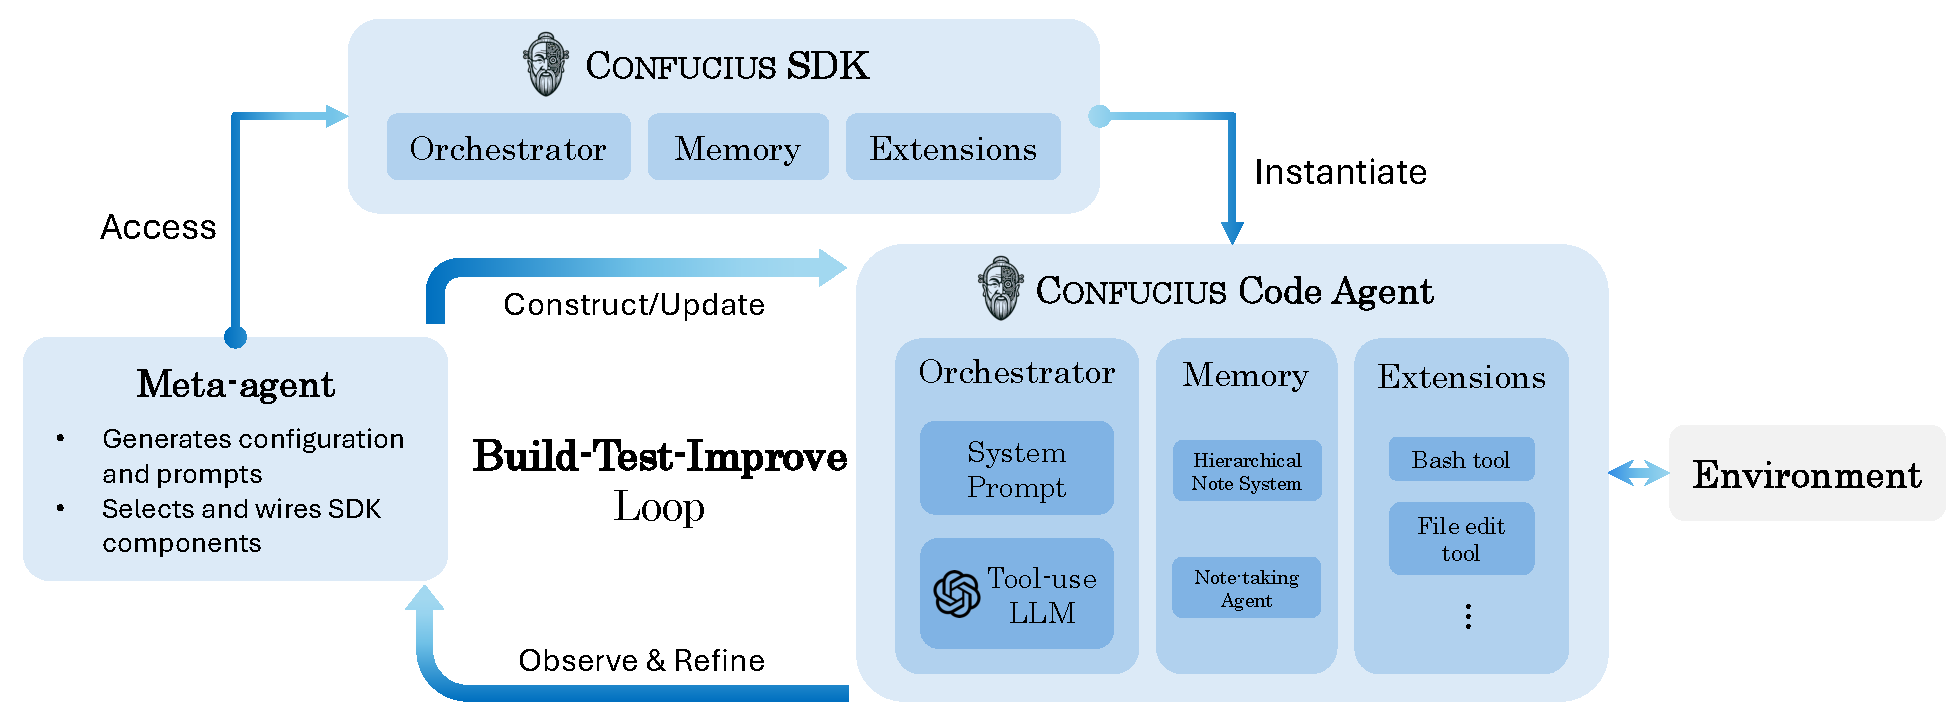
\includegraphics[width=\textwidth]{figs/meta_agent.pdf}
    \caption{\textbf{Meta-agent build–test–improve loop.} The Confucius Code Agent (CCA) is a specific agent built on top of the Confucius SDK, with the help of the meta-agent. The Meta-agent synthesizes agent configurations, wires together orchestrator components and extensions, evaluates candidate agents on representative tasks, and iteratively refines prompts and tool-use policies based on observed failures.}
    \label{fig:meta-agent}
\end{figure*}

As \Cref{fig:meta-agent} shows, the Meta-agent is implemented as an extra agent that interactively constructs new agents from high-level specifications based on the Confucius SDK. A developer begins by describing, in natural language, what the target agent should do and under what constraints (e.g., ``an agent that triages CI failures for our monorepo'' or ``a refactoring agent with read-only access to production configs''). The Meta-agent then generates a structured configuration form that asks for more concrete requirements: repository scope, latency or safety constraints, which existing extensions (file editing, bash, code search, etc.) to attach, and what evaluation tasks or test suites should be used. After the user confirms this specification, the Meta-agent automatically (i) synthesizes the agent’s configuration and prompts and (ii) wires in the selected extensions and memory policies. We present a brief illustration of this user interface in Appendix~\ref{sec.meta-agent-dev-cycle}.

Importantly, the Meta-agent also automates \emph{testing and debugging} of the newly created agent. Using the same SDK runtime, it spins up the candidate agent locally, drives it on a suite of regression tasks (e.g., representative GitHub issues or internal tickets), and observes the agent’s outputs, logs, and tool traces. When failures or undesirable behaviors are detected, such as brittle tool selection, incorrect file-edit patterns, or poor recovery from compiler errors, the Meta Agent proposes concrete modifications to prompts, extension configurations, or even new tool wrappers. These patches are applied to the agent, and the test loop is rerun, yielding a ``build-test-improve'' process that incrementally improves the agent until target metrics are met. The same mechanism can be invoked not only to build new agents, but also to assist in designing and debugging new tools that plug into the extension layer.


\subsection{Development Cycle}
\label{sec.meta-agent-dev-cycle}

The Confucius SDK promotes an easy-to-use \textbf{agent development cycle} where the meta-agent assist in onboarding and refining other agents.  
This iterative process of build-test-improve loop is further supported by a full suite of developer tools:  
\begin{itemize}[leftmargin=*]
\item \textbf{Onboarding Experience:} Meta-agent provides an easy-to-use interface for developers to create an agent from scratch, the onboarding experience offers multiple coding agent templates (orchestrators + extensions) and a multi-turn Q\&A session with developer to clarify requirements, it also offers E2E testing capabilities, where user can on-the-fly build test cases and optimize the agent code/prompt.
\item \textbf{Trace UI:} fine-grained visualization of call stacks, tool interactions, and memory flows, as shown in Figure~\ref{fig:trace_ui_v2}
\item \textbf{Playground:} an interactive environment for prompt refinement and parameter tuning;
\item \textbf{Eval UI:} built-in support for regression tests, A/B comparisons, and benchmark evaluations;
\item \textbf{Centralized agent management:} a unified interface for developing, integrating, deploying, and monitoring agents at scale.
\end{itemize}

\begin{figure}[h]
  \centering
  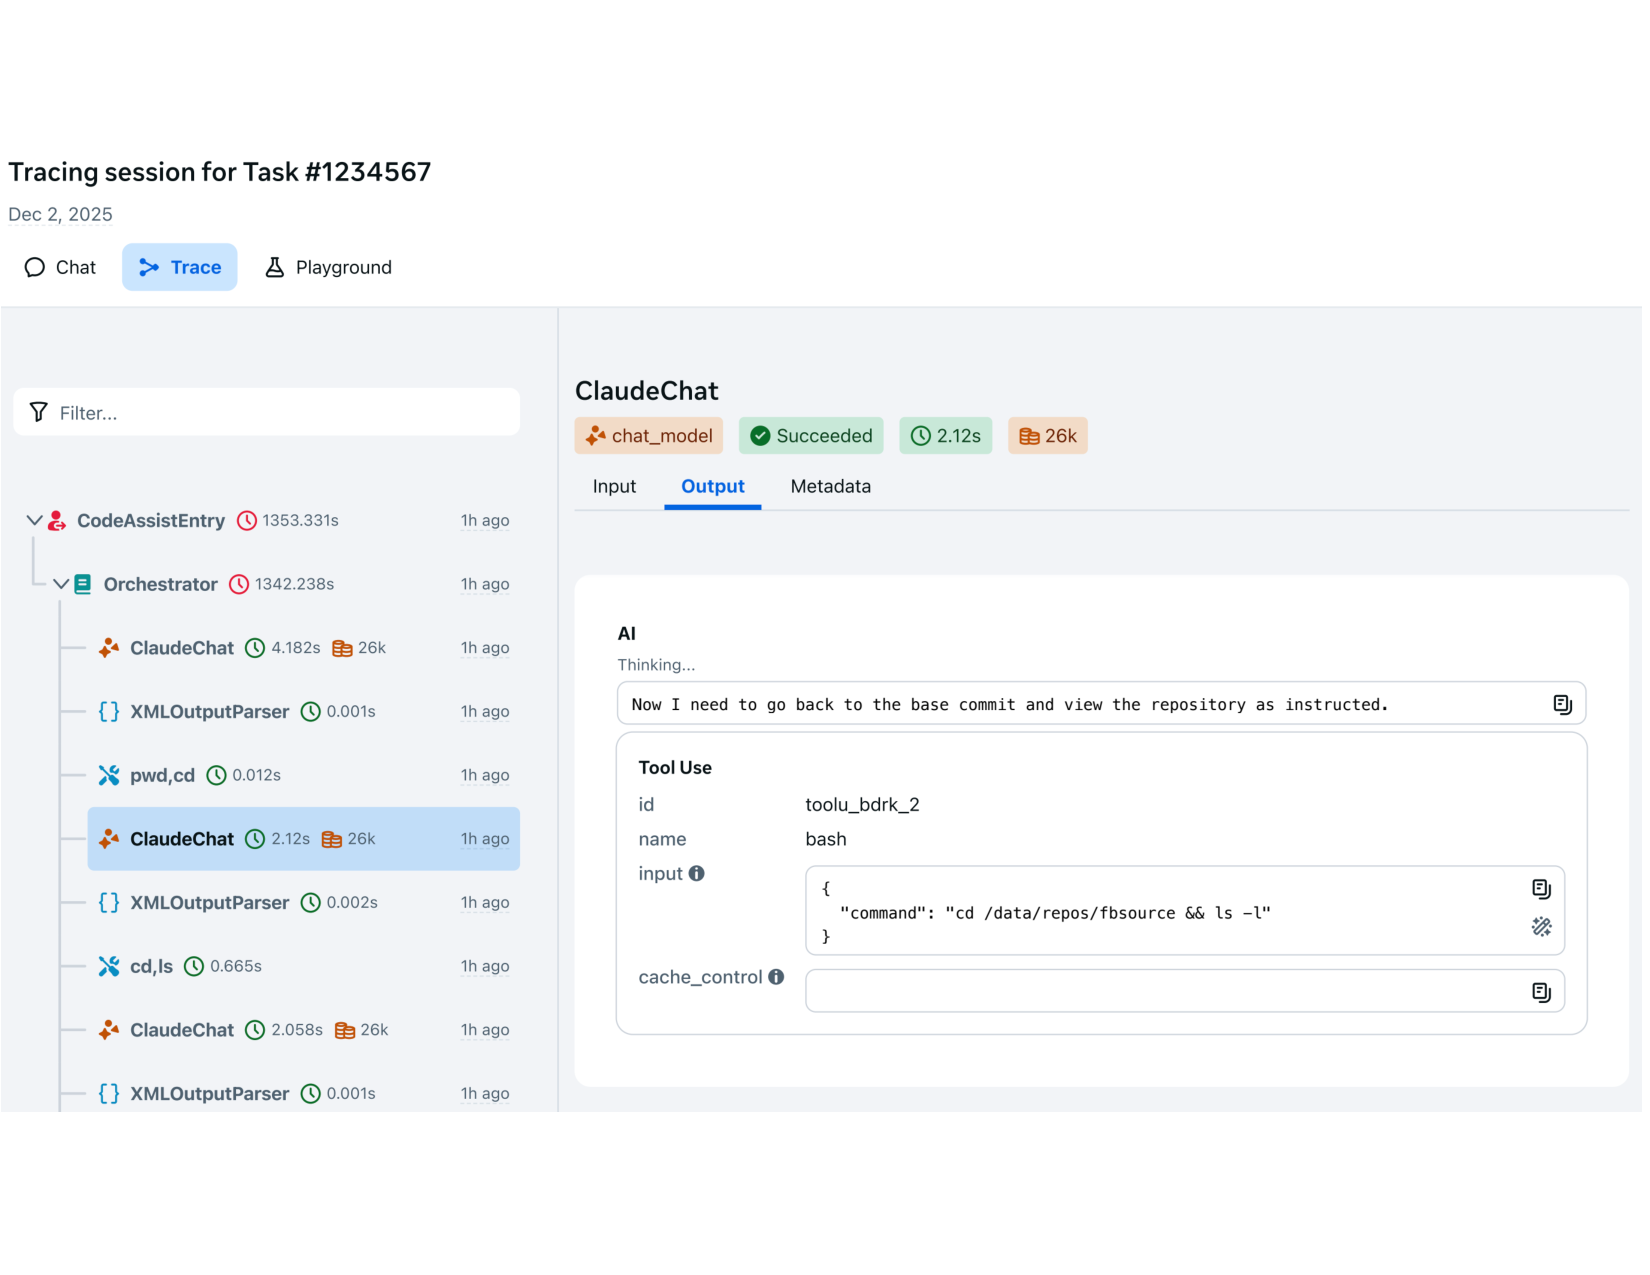
\includegraphics[width=\textwidth]{figs/trace_ui_v2.pdf}
  \caption{CCA Trace UI with call stack visualization and tool invocation Details, providing developers with detailed visibility into agent execution, showing the hierarchical call stack, latency metrics, token usage, and tool invocations for debugging and performance optimization. }
  \label{fig:trace_ui_v2}
\end{figure}


\section{Thinking Budget Scaling}
\label{app:thinking}
We define the \emph{thinking budget} as the maximum number of reasoning or chain-of-thought ``thinking'' tokens that the LLM is permitted to generate before producing a response. Recent work shows that reasoning length can be controlled by prompting or internal budget-aware mechanisms. At inference time, the model can be guided either by: (i) prompt instructions like ``use at most $X$ tokens of reasoning''~\citep{han2025token}; (ii) control tokens inserted periodically that signal remaining budget to the model during generation~\citep{wen2025budgetthinker}; or (iii) a predictor estimating task complexity and adjusting budget dynamically~\cite{li2025steering}. 

Anthropic's Claude model series expose a \texttt{thinkingBudget} parameter at inference time to directly cap the reasoning tokens. We run our CCA agent using Claude 4 Sonnet with identical setup except varying its thinking budget in three settings: $8$k, $16$k, and $32$k tokens. We record Resolve Rate on a subset of SWE-Bench-Verified.

\begin{table}[h]
\centering
\begin{tabular}{l c}
\toprule
\textbf{Thinking Budget} & \textbf{Resolve Rate (Pass@1)} \\
\midrule
8k   & 67.3 \\
16k  & 68.4 \\
32k  & 68.7 \\
\bottomrule
\end{tabular}
\caption{CCA Resolve Rate as a function of thinking budget on SWE-Bench-Verified subset.}
\label{tab:thinking_budget}
\end{table}

We observe diminishing returns beyond $16$k thinking tokens. Note that the \texttt{thinkingBudget} parameter cannot precisely control the internal thinking trace length of the Claude model, and that during inference, Claude only returns a summarized version of the reasoning without exposing full traces. As a result, we do not have the exact scaling curve of Resolve Rate with respect to the true thinking length on SWE-Bench-Verified.

\section{Example Execution Trace}
\label{app:trace}

Below, we show an example execution trace when running CCA on a SWE-Bench-Pro example: \texttt{instance\_tutao\_\_tutanota-da4edb7375c10f...}

\begin{tcolorbox}[colback=white,  % background color
                   colframe=black,    % frame color
                   coltext=metablue,      % text color
                   breakable,
                   fontupper=\scriptsize\fontfamily{pcr}\selectfont]  % font style and size
\begin{verbatim}
Running Confucius Code Agent with prompt from file: <PROMPT_FILE>

<SYSTEM>
Viewing directory at `<WORKDIR>`
Directory content viewed at `<WORKDIR>`, depth: 2, show_hidden: False

<AI>
The repository is in `<REPO_ROOT>`. Let me explore its structure:

<SYSTEM>
Viewing directory at `<REPO_ROOT_NAME>`
Directory content viewed at `<REPO_ROOT_NAME>`, depth: 2, show_hidden: False

<AI>
Let me search for `EntityRestClient` and related files:

<SYSTEM>
Validating command `find <REPO_ROOT> -type f -name "*.ts" | xargs grep -l "EntityRestClient" ... | head -20`
Running command in `<WORKDIR>`:
  find <REPO_ROOT> -type f -name "*.ts" | xargs grep -l "EntityRestClient" ... | head -20
Output:
  <REPO_ROOT>/src/api/common/EntityClient.ts
  <REPO_ROOT>/src/api/worker/rest/EntityRestClient.ts
  <REPO_ROOT>/src/api/worker/facades/BlobAccessTokenFacade.ts
  ...
Viewing file at `EntityRestClient.ts`
File content viewed at `EntityRestClient.ts`, lines: None - None

<AI>
Now let me search for `requestReadTokenArchive` and `requestReadTokenBlobs` in the codebase:

<SYSTEM>
Validating command `grep -rn "requestReadTokenArchive\|requestReadTokenBlobs" <REPO_ROOT>/src --include="*.ts"
...`
Running command in `<WORKDIR>`:
  grep -rn "requestReadTokenArchive\|requestReadTokenBlobs" <REPO_ROOT>/src --include="*.ts" ...
Output:
  <REPO_ROOT>/src/api/worker/facades/BlobAccessTokenFacade.ts:... requestReadTokenBlobs(...)
  <REPO_ROOT>/src/api/worker/facades/BlobAccessTokenFacade.ts:... requestReadTokenArchive(...)
  <REPO_ROOT>/src/api/worker/rest/EntityRestClient.ts:... requestReadTokenArchive(..., listId)
  ...

<SYSTEM>
Viewing file at `BlobAccessTokenFacade.ts`
File content viewed at `BlobAccessTokenFacade.ts`, lines: None - None

<AI>
Now let me look at the `createBlobAccessTokenPostIn` and related types to understand the structure:

<SYSTEM>
Validating command `grep -rn "createBlobAccessTokenPostIn\|BlobAccessTokenPostIn" <REPO_ROOT>/src 
--include="*.ts" ... | head -20`
Running command in `<WORKDIR>`:
  grep -rn "createBlobAccessTokenPostIn\|BlobAccessTokenPostIn" <REPO_ROOT>/src --include="*.ts" ... | head -20
Output:
  <REPO_ROOT>/src/api/entities/storage/TypeRefs.ts:... export type BlobAccessTokenPostIn = { ... }
  ...
Viewing file at `TypeRefs.ts`
File content viewed at `TypeRefs.ts`, lines: None - None

<AI>
(Problem analysis)
- `requestReadTokenArchive` / `requestReadTokenBlobs` currently require `archiveDataType`
- `EntityRestClient` hardcodes `ArchiveDataType.MailDetails`
- Requirement: allow `archiveDataType = null` for owned archives, keep behavior unchanged for non-owned
archives
...

<AI>
Now let me check the git status to see if there are any changes already made:

<SYSTEM>
Validating command `cd <REPO_ROOT> && git status`
Command rejected (disallowed): `cd ...`
Validating command `git -C <REPO_ROOT> status`
Running command in `<WORKDIR>`:
  git -C <REPO_ROOT> status
Output:
  HEAD detached from <COMMIT_SHA>
  nothing to commit, working tree clean

<AI>
This is a moderately complex task that involves changes to multiple files. Let me plan this out systematically.

<SYSTEM>
Writing to memory node 'todo.md'...
Created memory node 'todo.md' with ... characters and tags: ...

<AI>
Now let me create a reproduction script to understand the current behavior:

<SYSTEM>
Creating file at `reproduce.py`
File created successfully at `reproduce.py`

<AI>
Now let's run the reproduction script to confirm the issue:

<SYSTEM>
Validating command `python3 <REPO_ROOT>/reproduce.py`
Running command in `<WORKDIR>`:
  python3 <REPO_ROOT>/reproduce.py
Output:
  Test 1: ... archiveDataType allows null?  FAIL
  Test 2: ... method signatures accept null? FAIL
  Test 3: ... EntityRestClient passes null?  FAIL
  Some tests failed. The issue needs to be fixed.

<AI>
Implementing the fix.

<SYSTEM>
Replacing content in file at `TypeRefs.ts`
Diff:
  - archiveDataType: NumberString;
  + archiveDataType: NumberString | null;

<SYSTEM>
Replacing content in file at `BlobAccessTokenFacade.ts`
Diff:
  - requestReadTokenBlobs(archiveDataType: ArchiveDataType, ...)
  + requestReadTokenBlobs(archiveDataType: ArchiveDataType | null, ...)
  - requestReadTokenArchive(archiveDataType: ArchiveDataType, ...)
  + requestReadTokenArchive(archiveDataType: ArchiveDataType | null, ...)

<SYSTEM>
Replacing content in file at `EntityRestClient.ts`
Diff:
  - requestReadTokenArchive(ArchiveDataType.MailDetails, listId)
  + requestReadTokenArchive(null, listId)

<SYSTEM>
Replacing content in file at `EntityRestClient.ts`
Diff:
  - import { ArchiveDataType } from ".../TutanotaConstants.js"
  + (removed unused import)

<AI>
Now let's run the reproduction script again to verify the fix:

<SYSTEM>
Validating command `python3 <REPO_ROOT>/reproduce.py`
Running command in `<WORKDIR>`:
  python3 <REPO_ROOT>/reproduce.py
Output:
  Test 1: ... allows null, PASS
  Test 2: ... signatures accept null, PASS
  Test 3: ... passes null, PASS
  All tests passed! The fix is working correctly.

<AI>
Verifying diffs and committing.

<SYSTEM>
Validating command `git -C <REPO_ROOT> diff --name-only`
Running command in `<WORKDIR>`:
  git -C <REPO_ROOT> diff --name-only
Output:
  src/api/entities/storage/TypeRefs.ts
  src/api/worker/facades/BlobAccessTokenFacade.ts
  src/api/worker/rest/EntityRestClient.ts

<SYSTEM>
Validating command `git -C <REPO_ROOT> add -A && git -C <REPO_ROOT> commit -m "<COMMIT_MSG>"`
Running command in `<WORKDIR>`:
  git -C <REPO_ROOT> add -A && git -C <REPO_ROOT> commit -m "<COMMIT_MSG>"
Output:
  Committer: <ANON_NAME> <<ANON_EMAIL>>
  3 files changed, ... insertions(+), ... deletions(-)

<AI>
Done. Changes preserve existing behavior for non-owned archives, while allowing owned-archive read token 
requests without archiveDataType.
\end{verbatim}
\end{tcolorbox}




\section{Example Notes for Long-term Memory}
\label{app:notes}
Here is an example structured note hierarchy generated by note-taking agent for SWE-bench-Pro instance: \texttt{instance\_internetarchive\_\_openlibrary-f343c08f89c772f7ba...}.

\begin{tcolorbox}[colback=white,  % background color
                   colframe=black,    % frame color
                   coltext=metablue,      % text color
                   breakable,
                   fontupper=\scriptsize\fontfamily{pcr}\selectfont]  % font style and size
\begin{verbatim}
.
+-- projects
|   +-- openlibrary
|       +-- escaping_wildcards_in_infobase_queries.md
|       +-- multi_stage_author_matching_pipeline.md
|       +-- year_based_author_matching_strategy.md
+-- README.md
+-- shared
    +-- python
    |   +-- dict_copy_forgotten_field_update.md
    +-- string_manipulation
        +-- prefix_removal_empty_string_edge_case.md
\end{verbatim}
\end{tcolorbox}

The note is well organized into "shared" (ONLY for truly generic insights that apply across MANY projects) and "project" (For project-specific knowledge that primarily applies to ONE specific domain). The README.md summarized all the notes md files and provide instructions on how to navigate them. Here are some insights from \texttt{"escaping\_wildcards\_in\_infobase\_queries.md"}.

\begin{tcolorbox}[colback=white,  % background color
                   colframe=black,    % frame color
                   coltext=metablue,      % text color
                   breakable,
                   fontupper=\scriptsize\fontfamily{pcr}\selectfont]  % font style and size
\begin{verbatim}
---
id: escaping_wildcards_in_infobase_queries
title: Escaping Wildcards in Infobase Queries
description: How to handle asterisk characters in \\
Infobase queries to prevent unintended wildcard matching
keywords:
    - infobase
    - queries
    - wildcards
    - escaping
    - openlibrary
---

# Escaping Wildcards in Infobase Queries

## Problem Context

When searching for authors by name in OpenLibrary's Infobase, asterisk characters 
(`*`) in author names can cause unexpected behavior because they are treated as 
wildcards by the query system. For example, searching for an author named "John*" 
would match "John Smith", "Johnny", etc., rather than the literal name "John*". 


## The Solution

Escape asterisks in name fields using a backslash when performing exact or alternate 
name matches, but **intentionally preserve wildcards for surname matching queries**. 

### Code Example

```python
# In find_author() function:

# Escape asterisks for exact name matching
escaped_name = author["name"].replace("*", r"\*")

queries = [
    # Use escaped name for exact match
    {"type": "/type/author", "name~": escaped_name},
    # Use escaped name for alternate names
    {"type": "/type/author", "alternate_names~": escaped_name},
]

# For surname matching, intentionally use wildcards
if birth_year and death_year:
    surname = author['name'].split()[-1]
    queries.append({
        "type": "/type/author",
        "name~": f"* {surname}",  # Wildcard intentional here
        "birth_date~": f"*{birth_year}*",
        "death_date~": f"*{death_year}*",
    })
```

## Key Insights

1. **Context-Dependent Escaping**: Wildcards need to be escaped in some query contexts
(exact/alternate name matching) but preserved in others (surname matching).

2. **Backslash Escaping**: In Infobase queries, use `r"\*"` to escape asterisks. The
raw string `r` prefix prevents Python from interpreting the backslash.

3. **Query Order Matters**: The queries are tried in sequence. Exact matches (with
escaped wildcards) are tried first, then alternate names, then surname matching (with
intentional wildcards).

4. **Creating New Records**: When no match is found and a new author record must be
created, preserve the original name including any asterisks exactly as provided - 
don't use the escaped version.


## Related Files

- `/app/openlibrary/catalog/add_book/load_book.py` - `find_author()` function
- `/app/openlibrary/catalog/add_book/tests/test_load_book.py` - Tests for wildcard
behavior
\end{verbatim}
\end{tcolorbox}
These insights saves the agent a lot of effort to rediscover the issue in Run 2. 
Here are the insights from \texttt{prefix\_removal\_empty\_string\_edge\_case.md}.

\begin{tcolorbox}[colback=white,  % background color
                   colframe=black,    % frame color
                   coltext=metablue,      % text color
                   breakable,
                   fontupper=\scriptsize\fontfamily{pcr}\selectfont]  % font style and size
\begin{verbatim}
---
id: prefix_removal_empty_string_edge_case
title: Prefix Removal Empty String Edge Case
description: How to handle the edge case where removing a prefix leaves an empty string
keywords:
    - string
    - manipulation
    - edge
    - case
    - prefix
    - validation
---

# Prefix Removal Empty String Edge Case

## Problem

When removing a prefix from a string, you may end up with an empty string if the input
consists only of the prefix. This can cause unexpected behavior if downstream code
doesn't handle empty strings properly.

### Example Scenario

In OpenLibrary's honorific removal function, names like "Mr." or "Dr." consist 
entirely of an honorific:

```python
def remove_author_honorifics(author: dict[str, Any]) -> dict[str, Any]:
    raw_name: str = author["name"]
    
    if honorific := find_matching_honorific(raw_name):
        author["name"] = raw_name[len(honorific):].lstrip()
    return author
```

**Problem**: If `raw_name = "Mr."` and we remove "mr.", we get an empty string `""`,
which can cause issues in database queries or display logic.

## The Solution

Check if the result is empty after removing the prefix, and if so, return the original value unchanged:


```python
def remove_author_honorifics(author: dict[str, Any]) -> dict[str, Any]:
    """Remove honorifics from an author's name field."""
    raw_name: str = author["name"]
    
    # Check for exceptions first (e.g., "Dr. Seuss")
    if raw_name.casefold() in HONORIFC_NAME_EXECPTIONS:
        return author
    
    if honorific := next(
        (
            honorific
            for honorific in HONORIFICS
            if raw_name.casefold().startswith(honorific)
        ),
        None,
    ):
        new_name = raw_name[len(honorific):].lstrip()
        # If the name is only an honorific, return unchanged
        if not new_name:
            return author
        author["name"] = new_name
    return author
```

## Key Insights

1. **Check Before Assignment**: Store the result in a temporary variable and validate
it before assigning to the final location.

2. **Preserve Original on Invalid Result**: When validation fails (empty string),
return the original input unchanged rather than the invalid result.

3. **Common in Text Processing**: This pattern applies to any string manipulation
where you're removing parts of the string:
   - Removing file extensions
   - Removing URL protocols
   - Stripping whitespace/punctuation
   - Removing prefixes/suffixes
\end{verbatim}
\end{tcolorbox}

This documents a concrete edge case when solving the instance; this not only save the agent tokens in Run 2, but also avoid runs where in consecutive runs such edge cases could be missed hence fail the case.  

\section{Case Studies: Comparison with Claude Code}
\label{sec:case_studies}

In addition to standardized benchmarks, we conducted a controlled experiment using real GitHub issues from the PyTorch repository. These issues not only exemplify the complex challenges encountered in real-world production but also require deep domain specialist expertise. Hence, these issues reflect agent's robustness and generalization under specialist software engineering scenarios. Our experiment holds the model capabilities constant while varying only the agent framework. We compare \textbf{CCA} with \textbf{Claude Code (CC)}, a command-line tool developed by Anthropic that enables direct interaction with Claude models for coding tasks. Both frameworks utilize identical Claude Sonnet 4.5 models in environments with equivalent codebases and access to file manipulation, bash tools, and NVIDIA A100 80GB GPU resources. To compare the solution between CC and CCA, we have enlisted a few experts in this field to judge and compare the solutions created by the 2 agents.


\subsection{PyTorch-Bench}

To construct PyTorch-Bench, we scanned GitHub issues on the open-source PyTorch repository \citep{pytorch2025} from Jan 2025 to Jul 2025. We selected 8 issues that are reproducible on an NVIDIA A100 80 GB GPU and that provide actionable structure, including a detailed description, a reproduction script, and instructions for replication of the issue. Both agents receive the same system prompt, which instructs them to start from a clean commit, attempt to reproduce the issue first, stop if reproduction fails in the current environment, and verify any proposed fix. We show an example task below and discuss it in more detail in the following sections.

\begin{tcolorbox}[colback=white,  % background color
                   colframe=black,    % frame color
                   coltext=metablue,      % text color
                   breakable,
                   fontupper=\scriptsize\fontfamily{pcr}\selectfont]  % font style and size
\begin{verbatim}
Issue: RuntimeError: Expected curr_block->next == nullptr to be true,  when I call setSegmentStateToCheckpoint. 
(#161356)
URL: https://github.com/pytorch/pytorch/issues/161356

### Describe the bug

Hello, when I was using checkpoint state to implement shared output memory for two cudagraphs, an assert 
ERROR occurred:
curr_block->next == nullptr, in function setSegmentStateToCheckpoint.

```
# PyTorch version: 2.6.0+cu124

torch._C._cuda_setCheckpointPoolState(com_device, small_state, [], output1_new_storage)
RuntimeError: Expected curr_block->next == nullptr to be true, but got false.  
(Could this error message be improved?  If so, please report an enhancement request to PyTorch.)
'''

**This error only appears only when I set env `export PYTORCH_CUDA_ALLOC_CONF=expandable_segments:True`.
If I unset this env, the following case code executes successfully.**

This is my test code:
```
import gc
import torch
print(f"torch version is: {torch.__version__}.")
stream0 = torch.cuda.Stream()
torch.cuda.set_stream(stream0)

def tensor_metadata(x):
    return {
        "nbytes": x.untyped_storage().nbytes(),
        "data_ptr": x.untyped_storage().data_ptr(),
        "size": x.shape,
        "stride": x.stride(),
        "dtype": x.dtype,
        "device": x.device,
        "storage_offset": x.storage_offset(),}

def reconstruct_from_tensor_metadata(metadata):
    s = torch._C._construct_storage_from_data_pointer(
        metadata["data_ptr"], metadata["device"], metadata["nbytes"])
    t = torch.empty([0], device=metadata["device"], dtype=metadata["dtype"])
    t.set_(source=s, storage_offset=metadata["storage_offset"],
           size=metadata["size"], stride=metadata["stride"], )
    return t

def print_mem_stats(name):
    segments = torch.cuda.memory_snapshot()
    seg = []
    for segment in segments:
        if "segment_pool_id" in segment:
            tmp = ({"stream": segment["stream"]},
                   {"pool_id": segment["segment_pool_id"]},
                   {"block_num": len(segment["blocks"])},
                   {"activate_num": sum(int(blk["state"] == "active_allocated") for blk in segment["blocks"])},
                   {"total_size": segment["total_size"]},
                   {"allocated_size": segment["allocated_size"]},)
            seg.append(tmp)
    seg_str = "\n".join([str(seg_iter) for seg_iter in seg])
    seg_str = '\n' + seg_str
    print(f"{name}, snapshot: {seg_str}")

def cudagraphify(fn, inputs, pool, stream):
    torch.cuda.synchronize()
    gc.collect()
    torch.cuda.empty_cache()

    graph = torch.cuda.CUDAGraph()
    with torch.cuda.graph(graph, stream=stream, pool=pool):
        static_outputs = fn(*inputs)
    return graph, static_outputs


def foo(x, idx):
    r1 = x.expand([1, 2097152 // 8]).sqrt()
    r2 = x.expand([idx, 2097152]).clone()
    return (r1, r2)

# init
pool_id = torch.cuda.graph_pool_handle()
com_stream = torch.cuda.Stream()
com_device = torch.cuda.current_device()
inp = torch.tensor([7], device=com_device)

# record original state
with torch.cuda.stream(com_stream):
    g = torch.cuda.CUDAGraph()
    g.capture_begin(pool=pool_id)
    g.capture_end()
original_mem_state = torch._C._cuda_getCheckpointState(com_device, pool_id)

# start capture graph1
graph1, outputs1 = cudagraphify(foo, [inp, 1], pool=pool_id, stream=com_stream)
small_state = torch._C._cuda_getCheckpointState(com_device, pool_id)
print_mem_stats("\n-----------------after_small_state_run_g0_step0    ")
output1_metadata = [tensor_metadata(t) for t in outputs1]
outputs1 = None

# set to original state and capture graph2
torch._C._cuda_setCheckpointPoolState(com_device, original_mem_state, [], [])
print_mem_stats("\n-----------------after_set_origin_state     ")
graph2, outputs2 = cudagraphify(foo, [inp, 2], pool=pool_id, stream=com_stream)
biiig_state = torch._C._cuda_getCheckpointState(com_device, pool_id)
print_mem_stats("\n-----------------after_biiig_state_run_g1_step0    ")
output2_storage = [output.untyped_storage()._cdata for output in outputs2]

# set to original state and replay graph1
torch._C._cuda_setCheckpointPoolState(com_device, original_mem_state, output2_storage, [])
print_mem_stats("\n-----------------after_set_origin_state     ")
graph1.replay()
reconstructed_tensors1 = [reconstruct_from_tensor_metadata(metadata) for metadata in output1_metadata]
output1_new_storage = [output.untyped_storage()._cdata for output in reconstructed_tensors1]
torch._C._cuda_setCheckpointPoolState(com_device, small_state, [], output1_new_storage)
print_mem_stats("\n-----------------after_small_state_run_g0_step1    ")
```

After analyzing the error, the logic of the assertion seems to be: when allocing a new memory block, the last
block must be an unmapped 
nullptr block. Therefore, when setting to the recorded CheckpointState, the last block should also be unmapped
nullptr block.

Why does it fail only when enabling expandable_segments? It seems that after enabling expandable_segments, the 
reserved memory blocks 
will be merged. Therefore, when allocing a small block, releasing this small block, and then allocing a large
block again, the total reserved 
memory size increases. So, when setting to the state of a small memory block again, it triggers this assert 
error.

Could you please help check if these failed validations are always necessary? And how the current checkpoint 
memory management interface can solve the above problems when expandable_segments is enabled?  Thanks a lot.

### Versions

Collecting environment information...
PyTorch version: 2.6.0+cu124
Is debug build: False
CUDA used to build PyTorch: 12.4
ROCM used to build PyTorch: N/A

OS: Ubuntu 20.04.6 LTS (x86_64)
GCC version: (Ubuntu 9.4.0-1ubuntu1~20.04.3) 9.4.0
Clang version: Could not collect
CMake version: version 3.16.3
Libc version: glibc-2.31

Python version: 3.11.4 (main, Jul  5 2023, 13:45:01) [GCC 11.2.0] (64-bit runtime)
Python platform: Linux-5.15.0-72-generic-x86_64-with-glibc2.31
Is CUDA available: True
CUDA runtime version: 12.9.41
CUDA_MODULE_LOADING set to: LAZY
GPU models and configuration:
GPU 0: NVIDIA A100-SXM4-80GB
GPU 1: NVIDIA A100-SXM4-80GB
GPU 2: NVIDIA A100-SXM4-80GB
GPU 3: NVIDIA A100-SXM4-80GB
GPU 4: NVIDIA A100-SXM4-80GB
GPU 5: NVIDIA A100-SXM4-80GB
GPU 6: NVIDIA A100-SXM4-80GB
GPU 7: NVIDIA A100-SXM4-80GB

Nvidia driver version: 575.51.03
cuDNN version: Could not collect
HIP runtime version: N/A
MIOpen runtime version: N/A
Is XNNPACK available: True

\end{verbatim}
\end{tcolorbox}

\subsection{Issues and Comparative Solutions}

We present three representative cases that demonstrate divergent agent behaviors:

\textbf{CUDA Memory Checkpoint Assertion failure with Expandable Segments}

As shown above, PyTorch Issue \#161356 describes an error in PyTorch's CUDA graph checkpointing with expandable segments enabled. During a sequence that saves a small memory state, then a larger one, and restores the smaller state, PyTorch raises the error: ``Expected \small{\texttt{curr\_block->next == nullptr}} \normalsize to be true.'' Assertion failures occur in the allocator's checkpoint restoration logic, where terminal blocks in expandable segments are expected to have null next pointers.

Both frameworks identified the same underlying issue but proposed fundamentally different solutions. CCA viewed the assertions as overly restrictive and simply removed the problematic \small{\texttt{TORCH\_CHECK(curr\_block->next == nullptr)}} \normalsize assertions (--2 lines), while preserving other essential safety checks. CC viewed the assertions as important architectural guardrails and, instead of removing them, added logic (+7 lines) to explicitly set \small{\texttt{remaining->next = nullptr}} \normalsize during block splitting, effectively making expandable segments comply with the assertion. CCA favored minimal intervention, while CC pursued a more holistic solution. In this case, we note that the PyTorch team's eventual fix matched CCA's approach, providing human validation of CCA's principled engineering style.

\textbf{Excessive Memory Allocation and Deallocation during Llama-2 Training}

PyTorch Issue \#135837 highlights a memory allocation problem encountered during Llama-2 (70B) model Training. When GPU memory utilization approaches hardware limits, the allocator must decide whether to reclaim cached memory or retain it for performance optimization. On A100 GPUs (80GB), excessive memory deallocation and reallocation cycles occurred when reserved memory exceeded 70GB despite \small{\texttt{expandable\_segments=True}}, \normalsize resulting in significant Training slowdowns.

The issue was identified in PyTorch's CUDA allocator logic: even when the user explicitly enables expandable segments, the \small{\texttt{release\_cached\_blocks()}} \normalsize function continues to unmap expandable segments, causing unintended memory deallocation. This created a contradiction between user intent (maintaining expanded memory) and system behavior (aggressive memory reclamation). 

To solve this issue, CCA implemented a single guard clause (+6 lines) to fully disable memory reclamation when expandable segments are enabled, thus strictly adhering to the user's intent. In contrast, CC developed a more complex solution (+63 lines), dynamically measuring memory pressure and raising the reclamation threshold from 87.5\% to 95\%, while preserving emergency mechanisms above 95\% to prevent out-of-memory errors. Both solutions effectively addressed the immediate issue but reflected contrasting philosophies. CCA identified and minimally fixed the problematic behavior, while CC addressed the broader memory management challenge with a more sophisticated approach. 

\textbf{Neural Network Precision Regression during Weight Manipulation}

PyTorch Issue \#163072 involves a test failure where \small{\texttt{test\_partial\_flat\_weights}} \normalsize produces numerical accuracy errors on A100 and H100 GPUs, with relative differences of approximately 0.003 versus the expected tolerance of 1.3e-06. The test validates that partial flat weights (a memory optimization that stores select neural network layers in contiguous memory blocks) yield results equivalent to standard weight storage. The failure occurred during a sequence where LSTM weights were deleted, the module was moved to CUDA, and weights were manually restored. 

Both CCA and CC correctly identified the root cause as inappropriate test tolerances for GPU operations and  implemented the same adjustment: changing the tolerance parameters from exact equality to \small{\texttt{atol=1e-4,} \texttt{rtol=1e-4}} \normalsize (+1 line). This modification allowed the test to pass. 

However, CC did not stop there. While confirming that the adjusted test passes, CC encountered a benign warning about non-contiguous memory layout. In response, CC implemented additional changes (+20 lines), modifying \small{\texttt{setattr}} \normalsize in \small{\texttt{RNNBase}} \normalsize to automatically call \small{\texttt{flatten\_parameters()}} \normalsize whenever weights are manually assigned. Ultimately, CC addressed not only the immediate test failure but also the underlying warning, resulting in a more comprehensive but potentially over-engineered solution. 

\subsection{Architectural Analysis}

\begin{figure}[h]
  \centering
  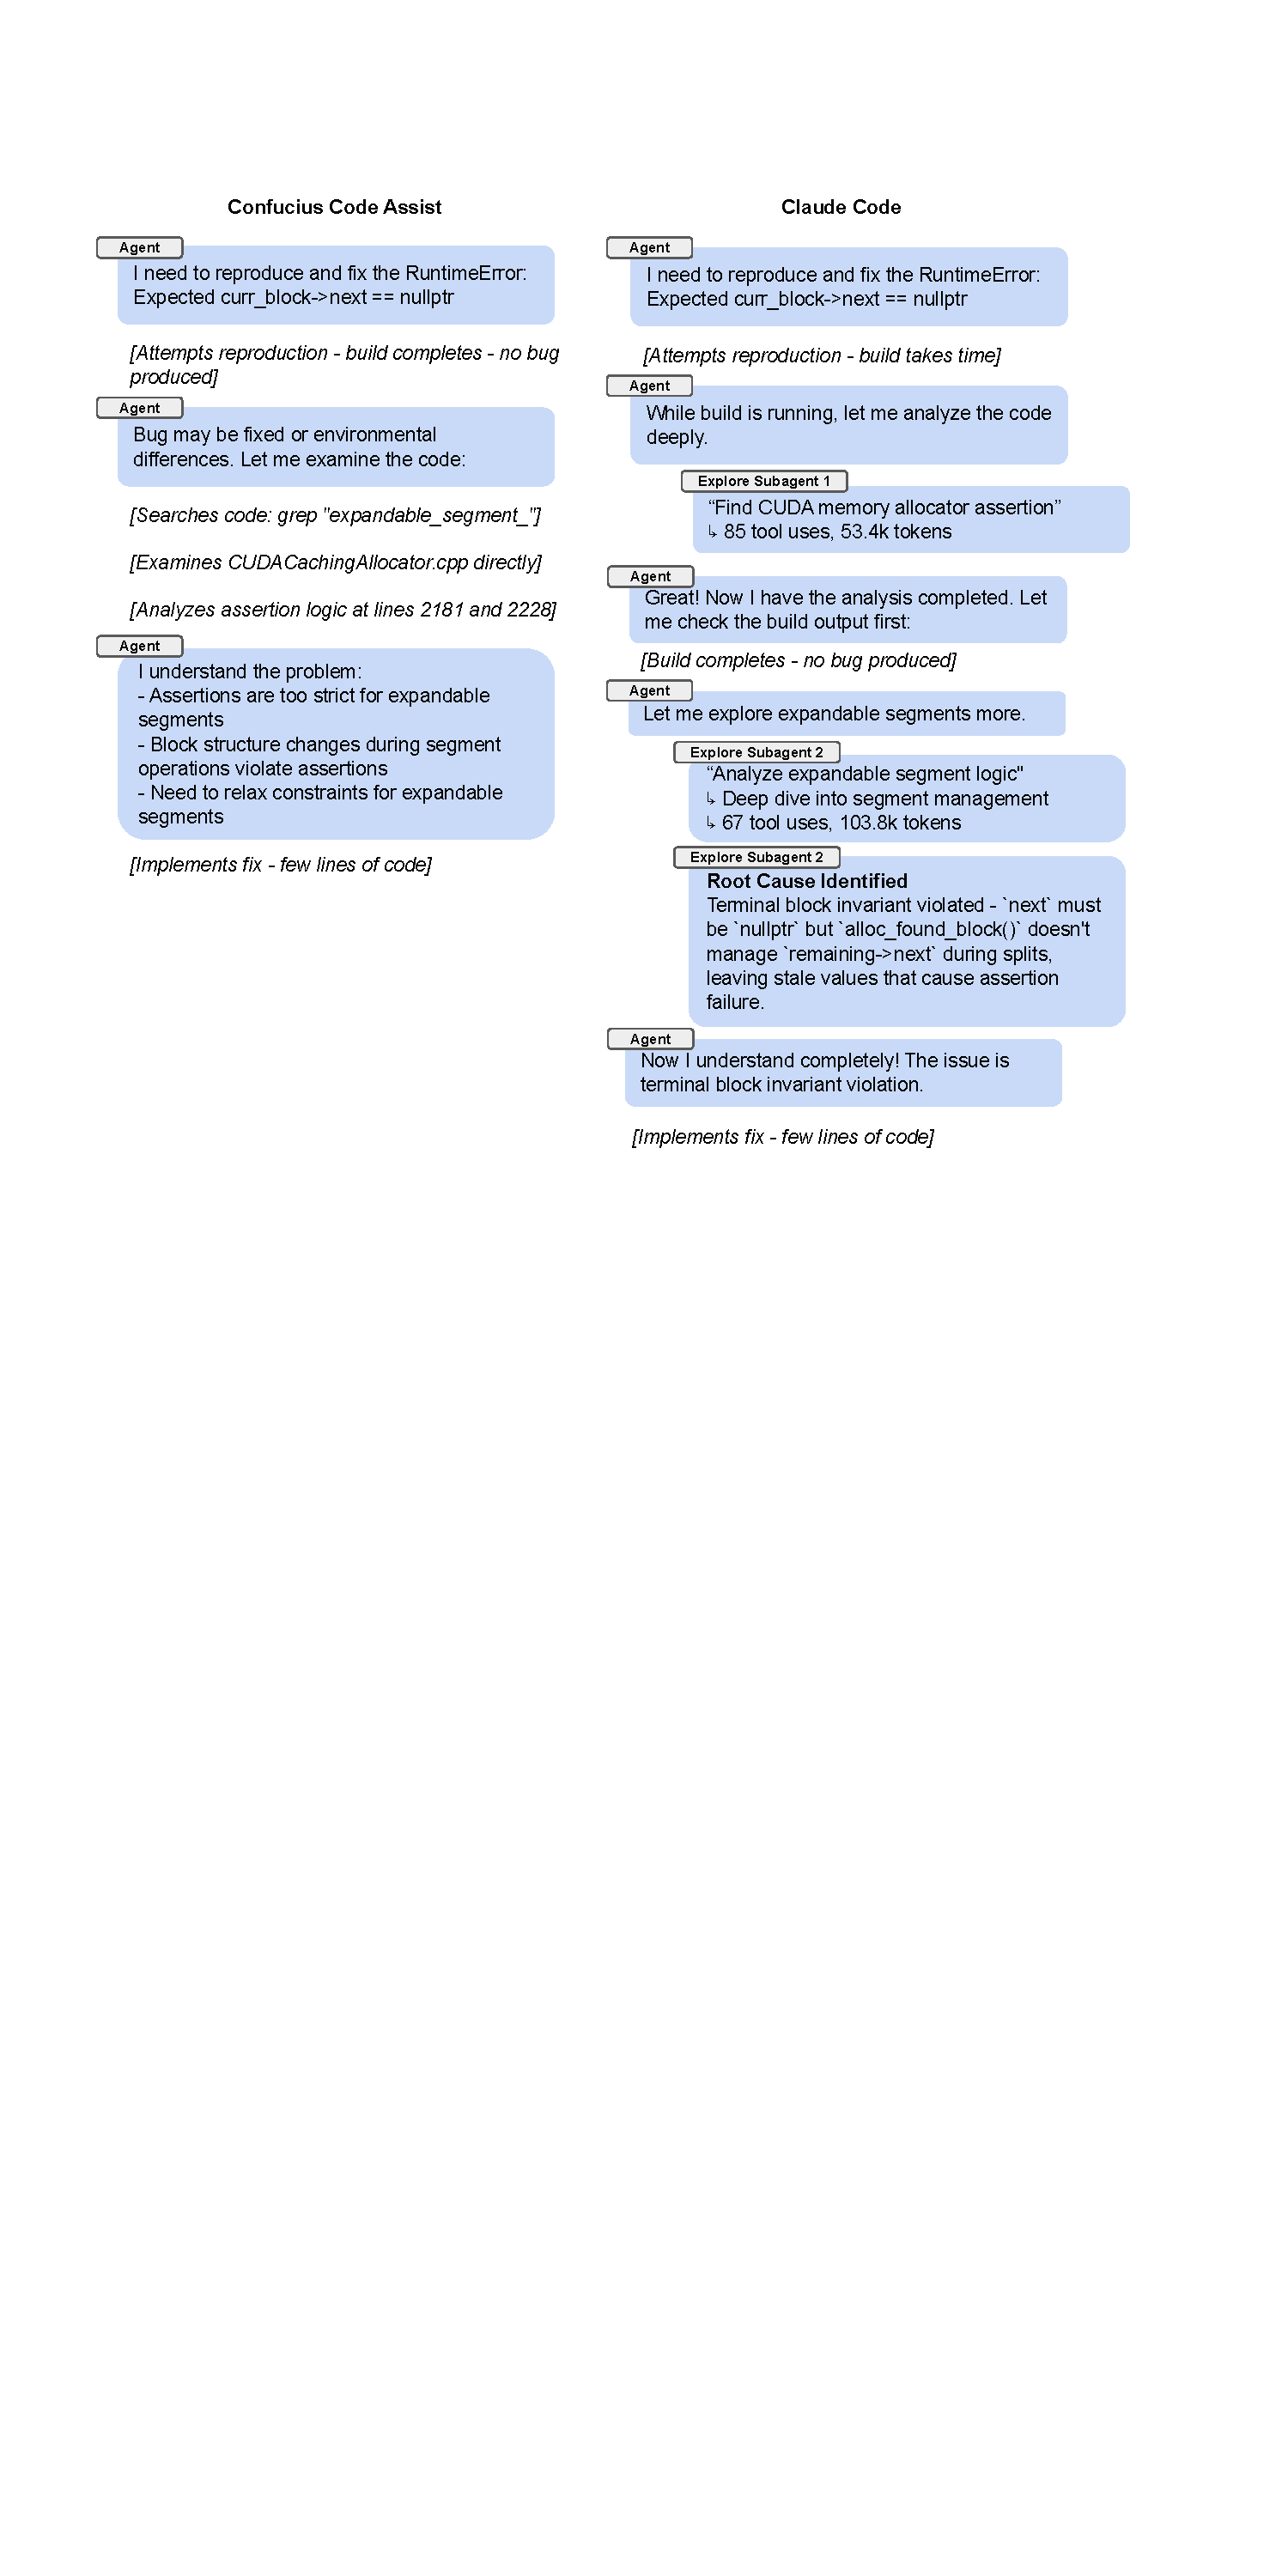
\includegraphics[width=0.8\textwidth]{figs/pytorch_traces.pdf}
  \caption{Simplified traces for CCA and CC on PyTorch issue \#161356}
  \label{fig:pytorch_traces}
\end{figure}

This section analyzes the problem-solving behavior of CCA versus CC on Issue \#161356. Figure~\ref{fig:pytorch_traces} shows simplified traces of the solutions of both agents. Both employed similar high-level strategies: (1) initial reproduction attempts, (2) code exploration when reproduction failed, (3) root cause identification through systematic analysis. 

Both agents also recognized the need for two directions of exploration: locating assertion failures in the CUDA memory allocator and understanding expandable segments logic. However, they perform these explorations differently: 
\begin{enumerate}
    \item \textbf{Single-Agent:} CCA performed explorations directly within the original context, maintaining awareness of the user's problem, system instructions, and previous observations. As such, CCA's explorations are subsequences of the overall reasoning chain.
    \item \textbf{Multi-Agent:} CC delegates investigations to separate, stateless subagents. As shown in Figure~\ref{fig:pytorch_traces},  CC even executes one of the subagents concurrently, while the main agent is running the reproduction script. These agents do not access the main agent's context, but they are initialized with a detailed prompt that emphasizes thoroughness (``use a thorough approach to find all relevant files''). 
\end{enumerate}

The architectural differences between CCA and CC significantly influenced solution characteristics. CCA's solution was simpler and more cautious, whereas CC was more ambitious and overengineered its solution. CC opted for this solution because it was the suggestion returned by the subagent, which was tasked with performing an exhaustive analysis. The subagent's mandate for thoroughness, combined with its lack of the original context, leads it to over-analyze the problem and provide a more complex solution than is necessary. The main agent, trusting the subagent's expertise, implements the solution despite preferring simpler solutions independently. This highlights a fundamental challenge in multi-agent systems. Generally, subagents separate concerns and allow the main agent to focus on its main task. However, our analysis suggests that for well-scoped debugging tasks, the benefits of delegation may be outweighed by the risk of context loss and derailment via inter-agent misalignment.


\section{Future Work}

Recent advances suggest that reinforcement learning (RL) can substantially enhance LLM-based software engineering agents beyond what is achievable with supervised fine-tuning alone. For example, SWE-RL~\citep{wei2025swe} demonstrates meaningful gains through end-to-end RL with verifiable rewards, while frameworks such as Agent Lightning~\citep{luo2025agentlightningtrainai} highlight a crucial architectural insight: by viewing agent execution as a Markov Decision Process, RL training can be decoupled from agent implementation via unified trajectory interfaces.
This decoupled perspective aligns naturally with the design philosophy behind CCA. The Agent Experience (AX) framework already structures an agent’s internal reasoning traces in a trajectory-friendly format, making them directly suitable for RL training. Moreover, CCA’s Meta-agent produces rich, fine-grained feedback signals from both tool extensions and environment interactions—signals that can be transformed into diverse reward functions for outcome-based, process-based, or hybrid supervision. Examples include rewards tied to note-taking quality, tool-use robustness, recovery behaviors, or the efficiency of multi-step exploration.
In addition, the extensibility of the Confucius Orchestrator provides a natural substrate for curriculum design in RL. Agent builders can introduce progressively richer toolsets, varied execution environments (e.g., shell, file editing, SQL databases), and increasingly complex tasks, enabling models to acquire generalizable agentic capabilities rather than overfitting to specific tool behaviors. This opens the door to RL-driven improvement not only of individual policies, but of the broader agent stack itself.


\clearpage


